%%
%% Generated by gpt_translate from test/images.tex, on 2024-07-09 16:43:18 using model gpt-3.5-turbo-16k
%%

% GPT CHUNK%
\documentclass{ximera}
% ../preamble.tex
% \addPrintStyle{..}

\begin{document}
    \xmtitle{Images}{}

    \providecommand{\psize}[1]{
        \pgfmathparse{#1}
        \pgfmathresult pt
    }
    
    A tikzpicture without anything else:
        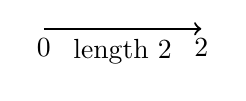
\begin{tikzpicture}
            \draw[thick,->]
            (0,0) node[below] {$0$} 
              --  node[below] {length 2}
            (2,0) node[below] {$2$};
        \end{tikzpicture}

    A tikzpicture inside a \verb|\begin{tikzpicture}[scale=2]|.
        \begin{tikzpicture}[scale=2]
            \draw[thick,->]
            (0,0) node[below] {$0$} 
              --  node[below] {length 2}
            (2,0) node[below] {$2$};
        \end{tikzpicture}

    A tikzpicture inside a \verb|\begin{tikzpicture}[scale=0.5]|.
        \begin{tikzpicture}[scale=0.5]
            \draw[thick,->]
            (0,0) node[above] {$0$} 
              --  node[below] {length 2}
            (2,0) node[above] {$2$};
        \end{tikzpicture}

 A tikzpicture inside a \verb|\begin{image}[1cm]| with size =\psize{1cm}.
    \begin{image}[1cm]
        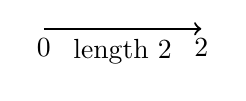
\begin{tikzpicture}
            \draw[thick,->]
            (0,0) node[below] {$0$} 
              --  node[below] {length 2}
            (2,0) node[below] {$2$};
        \end{tikzpicture}
    \end{image}

    A tikzpicture inside a \verb|\begin{image}[\textwidth]| with size =\psize{\textwidth} (and textwidth =\the\textwidth).

    \begin{image}[\textwidth]
        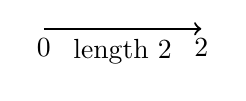
\begin{tikzpicture}
            \draw[thick,->]
            (0,0) node[below] {$0$} 
              --  node[below] {length 2}
            (2,0) node[below] {$2$};
        \end{tikzpicture}
    \end{image}

    A tikzpicture inside a \verb|\begin{image}[0.5\textwidth]| with size =\psize{0.5\textwidth}.
    \begin{image}[0.5\textwidth]
        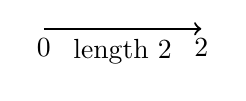
\begin{tikzpicture}
            \draw[thick,->]
            (0,0) node[below] {$0$} 
              --  node[below] {length 2}
            (2,0) node[below] {$2$};
        \end{tikzpicture}
    \end{image}

    A tikzpicture inside a \verb|\begin{image}[0.2\textwidth]| with size =\psize{0.2\textwidth}.
    \begin{image}[0.2\textwidth]
        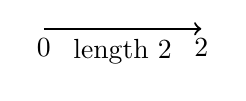
\begin{tikzpicture}
            \draw[thick,->]
            (0,0) node[below] {$0$} 
              --  node[below] {length 2}
            (2,0) node[below] {$2$};
        \end{tikzpicture}
    \end{image}

    A tikzpicture inside a \verb|\begin{image}[10cm]| with size =\psize{10cm}.
    \begin{image}[10cm]
        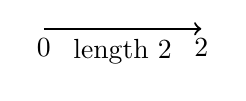
\begin{tikzpicture}
            \draw[thick,->]
            (0,0) node[below] {$0$} 
              --  node[below] {length 2}
            (2,0) node[below] {$2$};
        \end{tikzpicture}
    \end{image}

    A tikzpicture inside a \verb|\begin{image}[5cm]| with size =\psize{5cm}.
    \begin{image}[5cm]
        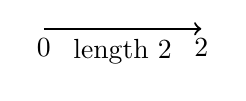
\begin{tikzpicture}
            \draw[thick,->]
            (0,0) node[below] {$0$} 
              --  node[below] {length 2}
            (2,0) node[below] {$2$};
        \end{tikzpicture}
    \end{image}

    A tikzpicture inside a \verb|\begin{image}[1cm]| with size =\psize{1cm}.
    \begin{image}[1cm]
        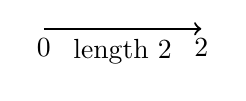
\begin{tikzpicture}
            \draw[thick,->]
            (0,0) node[below] {$0$} 
              --  node[below] {length 2}
            (2,0) node[below] {$2$};
        \end{tikzpicture}
    \end{image}

          

    \end{document}